\documentclass[]{elsarticle} %review=doublespace preprint=single 5p=2 column
%%% Begin My package additions %%%%%%%%%%%%%%%%%%%
\usepackage[hyphens]{url}

  \journal{Journal of Human Evolution} % Sets Journal name


\usepackage{lineno} % add
\providecommand{\tightlist}{%
  \setlength{\itemsep}{0pt}\setlength{\parskip}{0pt}}

\usepackage{graphicx}
\usepackage{booktabs} % book-quality tables
%%%%%%%%%%%%%%%% end my additions to header

\usepackage[T1]{fontenc}
\usepackage{lmodern}
\usepackage{amssymb,amsmath}
\usepackage{ifxetex,ifluatex}
\usepackage{fixltx2e} % provides \textsubscript
% use upquote if available, for straight quotes in verbatim environments
\IfFileExists{upquote.sty}{\usepackage{upquote}}{}
\ifnum 0\ifxetex 1\fi\ifluatex 1\fi=0 % if pdftex
  \usepackage[utf8]{inputenc}
\else % if luatex or xelatex
  \usepackage{fontspec}
  \ifxetex
    \usepackage{xltxtra,xunicode}
  \fi
  \defaultfontfeatures{Mapping=tex-text,Scale=MatchLowercase}
  \newcommand{\euro}{€}
\fi
% use microtype if available
\IfFileExists{microtype.sty}{\usepackage{microtype}}{}
\bibliographystyle{elsarticle-harv}
\usepackage{longtable}
\usepackage{graphicx}
\ifxetex
  \usepackage[setpagesize=false, % page size defined by xetex
              unicode=false, % unicode breaks when used with xetex
              xetex]{hyperref}
\else
  \usepackage[unicode=true]{hyperref}
\fi
\hypersetup{breaklinks=true,
            bookmarks=true,
            pdfauthor={},
            pdftitle={Ecological perspectives on technological diversity at Kanjera South},
            colorlinks=false,
            urlcolor=blue,
            linkcolor=magenta,
            pdfborder={0 0 0}}
\urlstyle{same}  % don't use monospace font for urls

\setcounter{secnumdepth}{0}
% Pandoc toggle for numbering sections (defaults to be off)
\setcounter{secnumdepth}{0}

% Pandoc citation processing
\newlength{\cslhangindent}
\setlength{\cslhangindent}{1.5em}
\newlength{\csllabelwidth}
\setlength{\csllabelwidth}{3em}
% for Pandoc 2.8 to 2.10.1
\newenvironment{cslreferences}%
  {}%
  {\par}
% For Pandoc 2.11+
\newenvironment{CSLReferences}[2] % #1 hanging-ident, #2 entry spacing
 {% don't indent paragraphs
  \setlength{\parindent}{0pt}
  % turn on hanging indent if param 1 is 1
  \ifodd #1 \everypar{\setlength{\hangindent}{\cslhangindent}}\ignorespaces\fi
  % set entry spacing
  \ifnum #2 > 0
  \setlength{\parskip}{#2\baselineskip}
  \fi
 }%
 {}
\usepackage{calc}
\newcommand{\CSLBlock}[1]{#1\hfill\break}
\newcommand{\CSLLeftMargin}[1]{\parbox[t]{\csllabelwidth}{#1}}
\newcommand{\CSLRightInline}[1]{\parbox[t]{\linewidth - \csllabelwidth}{#1}\break}
\newcommand{\CSLIndent}[1]{\hspace{\cslhangindent}#1}

% Pandoc header
\usepackage{booktabs}
\usepackage{longtable}
\usepackage{array}
\usepackage{multirow}
\usepackage{wrapfig}
\usepackage{float}
\usepackage{colortbl}
\usepackage{pdflscape}
\usepackage{tabu}
\usepackage{threeparttable}
\usepackage{threeparttablex}
\usepackage[normalem]{ulem}
\usepackage{makecell}
\usepackage{xcolor}



\begin{document}
\begin{frontmatter}

  \title{Ecological perspectives on technological diversity at Kanjera
South}
    \author[Max Planck Institute For Evolutionary Anthropology]{Jonathan
S. Reeves}
   \ead{Jonathan\_Reeves@eva.mpg.de} 
    \author[The George Washington University]{David R. Braun}
  
    \author[Max Plank Institute For the Science of Human History]{Emma
M. Finestone}
  
    \author[Queens College City University of New York]{Thomas W.
Plummer}
  
      \address[MPI]{Technological Primates Research Group, Max Planck
Institute For Evolutionary Anthropology, Deutscher Platz 6, Leipzig,
04103, Germany}
    \address[CASHP]{Center for the Advanced Study of Human Paleobiology,
George Washington University, 800 22nd Street, North West, Washington,
D.C., USA}
    \address[SHH]{Department of Archaeology, Max Planck Institute for
the Science of Human History, Kahlaische Strasse 10, Jena, D-07743,
Germany}
    \address[NYCEP]{Dept of Anthropology, Queens College, City
University of New York, Flushing, NY, 11367-1597, USA}
    
  \begin{abstract}
  The aspects of hominin behavior responsible for Oldowan stone tool
  variation are the focus of much debate. There is some consensus that
  this variation arises from a combination of ecological and cultural
  factors. The diversity of raw material types and technological
  strategies present at Kanjera South, Kenya, provide an opportunity to
  examine the interacting influences of ecology and culture on Oldowan
  stone tool variation. Here, we combine previous analyses of raw
  material properties, provenance, and technology with quantitative
  measures of core reduction intensity and tool utilization to examine
  the influence of both ecological and technocultural factors on stone
  tool variation at Kanjera South. The results of this analysis reflect
  a dynamic relationship between raw material properties, provenance,
  and hominin mobility. Exotic raw materials are generally more
  resistant to edge attrition compared with those available locally,
  which may have incentivized their transport over long distances and
  more extensive reduction. Cores produced on raw materials from distant
  sources also exhibit more complex core reduction strategies than
  locally acquired materials. While this pattern is partially due to the
  differences in the quality of knappable stone, bifacial centripetal
  and multifacial core reduction strategies also arise due to the
  continuous transport and use of exotic raw materials. Moreover, the
  variation in stone tool reduction is not consistent with neutral
  models of stone tool transport and discard. These results demonstrate
  that ecological factors such as raw material provenance and physical
  properties have strong impacts on reduction intensity and the
  technological strategies used by hominins.
  \end{abstract}
  
 \end{frontmatter}

\hypertarget{introduction}{%
\section{1. Introduction}\label{introduction}}

Upon its initial discovery, the Oldowan was considered an expedient
industry that was akin to simply smashing stones. Nearly a century
later, the Oldowan is now known to reflect a complex behavioral pattern
that encompasses not only the technical capacity to efficiently produce
flakes but also dynamic patterns of tool transport. Technological
analyses show that Oldowan hominins had at least a basic understanding
of the general principles of flaking and selection of suitable tool
stones for artifact manufacture (Semaw, 2000; de la Torre, 2004;
Delagnes and Roche, 2005; Stout et al., 2005; Toth and Schick, 2006;
Braun et al., 2009, 2019; Goldman-Neuman and Hovers, 2012). This pattern
of tool production was integrated into a broader land-use strategy in
which raw material was acquired, transported, used, maintained, and
eventually discarded (\hspace{0pt}Isaac and Harris, 1975\hspace{0pt};
\hspace{0pt}Hay, 1976\hspace{0pt}; \hspace{0pt}Isaac, 1981\hspace{0pt},
\hspace{0pt}1984\hspace{0pt}; \hspace{0pt}Toth, 1985\hspace{0pt},
\hspace{0pt}1987\hspace{0pt}; \hspace{0pt}Schick, 1987\hspace{0pt};
\hspace{0pt}Potts, 1991\hspace{0pt}, \hspace{0pt}1994\hspace{0pt};
\hspace{0pt}Blumenschine and Peters, 1998\hspace{0pt}; \hspace{0pt}Potts
et al., 1999\hspace{0pt}; \hspace{0pt}Blumenschine et al.,
2008\hspace{0pt}; \hspace{0pt}Braun et al., 2008a\hspace{0pt}). Although
these actions remained simple, the various ways in which they were
combined reflect a variety of production strategies that can be
evaluated on a site-by-site basis (\hspace{0pt}Delagnes and Roche,
2005\hspace{0pt}).

Research has revealed a wide range of technological diversity in the
Oldowan across time and space. A primary objective of current Oldowan
research is identifying the behavioral processes that shaped such a
diversity of production strategies (\hspace{0pt}Plummer,
2004\hspace{0pt}; \hspace{0pt}Roche et al., 2009\hspace{0pt};
\hspace{0pt}Gallotti, 2018\hspace{0pt}). A multitude of work now links
the technical diversity of the Oldowan to the cognition, skill, social
transmission of information, and, in some cases, social learning
mechanisms of Plio-Pleistocene hominins (\hspace{0pt}Schick and Toth,
1994\hspace{0pt}; \hspace{0pt}Stout and Chaminade, 2009\hspace{0pt};
\hspace{0pt}Hovers, 2009\hspace{0pt}, \hspace{0pt}2012\hspace{0pt};
\hspace{0pt}Stout, 2011\hspace{0pt}; \hspace{0pt}Goldman-Neuman and
Hovers, 2012\hspace{0pt}; \hspace{0pt}Roche et al., 2018\hspace{0pt};
\hspace{0pt}Toth and Schick, 2018\hspace{0pt}; \hspace{0pt}Stout et al.,
2019\hspace{0pt}). However, while our understanding of technical
decision-making has dramatically increased, research focusing on
ecological influences on Oldowan technological diversity, such as land
use and tool transport, has waned in recent decades (\hspace{0pt}de
Torre and Mora, 2009\hspace{0pt}).

Although stone tool diversity is linked to constraints imposed by raw
material geometry, quality, and abundance (\hspace{0pt}Toth,
1982\hspace{0pt}, \hspace{0pt}1985\hspace{0pt},
\hspace{0pt}1987\hspace{0pt}; \hspace{0pt}Potts, 1988\hspace{0pt},
\hspace{0pt}1991\hspace{0pt}; \hspace{0pt}de la Torre, 2004\hspace{0pt};
\hspace{0pt}Blumenschine et al., 2008\hspace{0pt}; \hspace{0pt}Braun et
al., 2009a\hspace{0pt}), how hominin tool transport and more broadly
land-use patterns influence the technical decision-making of Oldowan
tool makers remains unclear. Early work on this subject suggested that
Oldowan technological diversity reflects a continuum of reduction as
stone is moved across the landscape (\hspace{0pt}Toth, 1985\hspace{0pt};
\hspace{0pt}Potts, 1991\hspace{0pt}). While \hspace{0pt}Potts
(1991)\hspace{0pt} illustrated an interesting relationship between mass
and Leakey's typological core categories, little work has been done to
further establish connections between hominin land use and technological
diversity.

The \textasciitilde2.0 Ma site of Kanjera South contributes to our
understanding of the relationship between stone tool production,
technical decision-making, and hominin behavioral ecology. The lithic
assemblage at Kanjera South shows a substantial representation of exotic
raw materials (e.g., rock types not available within 10 km of the
archaeological site) and a diversity of different core reduction
strategies that provide an opportunity to understand the technical
decision-making within the context of broader hominin land-use
strategies. Although early Oldowan assemblages dating to 2.0 Ma and
older illustrate a similar level of technological competence to those
from later time frames, substantially less is known about the broader
foraging behaviors and land-use strategies of hominins during this
interval. An investigation of hominin stone tool transport and
utilization patterns at Kanjera would not only add to our understanding
of how the landscape structures stone tool use and transport but also
further elucidate the relationship between Oldowan technological
strategies and land use.

To this end, we present a new study of the Kanjera South lithic material
that combines previous analyses of raw material properties, provenance,
and technology with quantitative measures of core reduction intensity
and tool utilization to elucidate the broader land-use pattern. We show
that the technological variation at Kanjera South reflects an
interaction of raw material properties, foraging ecology, and landscape
scale constraints on raw material availability. We further characterize
the broader pattern of land use of Oldowan hominins at Kanjera South and
show that this pattern may condition the economization of stone
resources across space. This study sheds light on the environmental and
technical variables that contribute to Oldowan stone tool variability
and provides unique insight into hominin land-use patterns in the early
Oldowan.

\hypertarget{background-to-kanjera-south}{%
\subsection{1.1 Background to Kanjera
South}\label{background-to-kanjera-south}}

The \textasciitilde2.0 Ma site of Kanjera South is situated on the
northeastern side of the Homa Peninsula on the edges of the Nyanza Rift
near the shores of Lake Victoria (Plummer et al. (1999); Ditchfield et
al. (2019), Fig. \ref{map}). The extensive excavation of a 3-m-deep
sequence of silts and clays recovered more than 3000 fossils and more
than 4000 stone artifacts (\hspace{0pt}Plummer et al.,
2009a\hspace{0pt}). Spatially associated artifacts and fossils are found
as both diffuse scatters and vertically discrete horizons throughout
this sequence. Although the bulk of the archaeological sample is derived
from a single package of sediment called KS-2 (\hspace{0pt}Plummer and
Bishop, 2016\hspace{0pt}), the large number of artifacts recovered
throughout the sequence suggests that the site was repeatedly visited
over the course of this interval (\hspace{0pt}Ferraro et al.,
2013\hspace{0pt}). The stratigraphy at Kanjera South is made up of
approximately 30 m of fluvial, colluvial, and lacustrine sediments
(\hspace{0pt}Ditchfield et al., 2019\hspace{0pt}). Extensive research on
the geochronology and sedimentary context has demonstrated that the
lithics and fossils accumulated predominantly by hominin activity
(\hspace{0pt}Behrensmeyer et al., 1995\hspace{0pt}; \hspace{0pt}Plummer
et al., 2009a\hspace{0pt}, \hspace{0pt}2009b\hspace{0pt};
\hspace{0pt}Ferraro et al., 2013\hspace{0pt}; \hspace{0pt}Ditchfield et
al., 2019\hspace{0pt}).

\begin{figure}
\centering
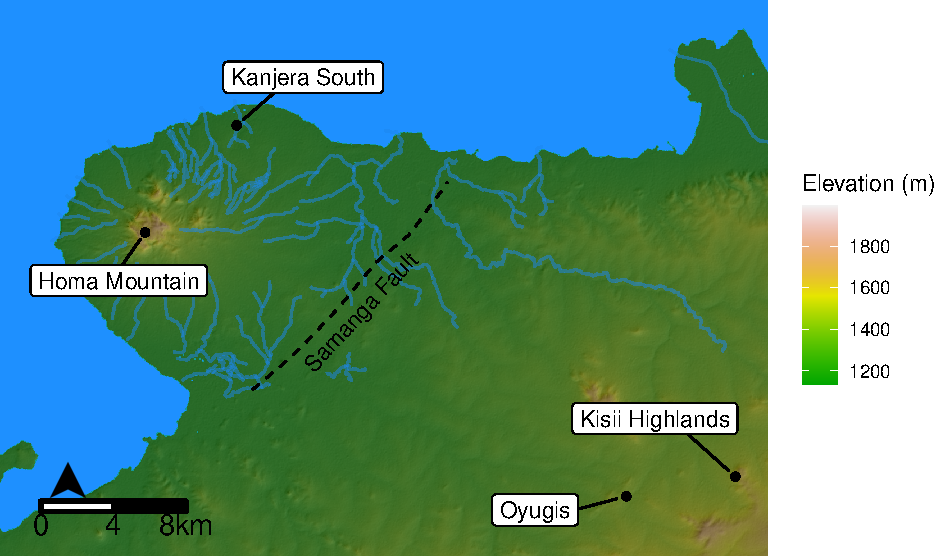
\includegraphics{Kanjera_South_Manuscript_files/figure-latex/fig-1-1.pdf}
\caption{A map of the Homa Peninsula. Kanjera South is situated to the
east of Homa Mountain. The Homa Mountain carbonatite center is the
primary source of the local raw materials including Homa limestone, Homa
phonolite, and fenetized Nyanzian rocks. Drainages coming off the flanks
of Homa Mountain carry these local rock types to within the immediate
vicinity of Kanjera South. Distant or exotic raw materials originate in
river conglomerates much farther to the east of the Samanga Fault. These
include Bukoban andesite, Bukoban felsite, Bukoban quartzite, Nyanzian
rhyolite, and Oyugis granite. \label{map}}
\end{figure}

The frequencies of different bovids and enamel isotope studies indicate
that the landscape surrounding Kanjera South, unlike the setting of many
Oldowan sites, was dominated by a grassland as opposed to more closed
habitats (\hspace{0pt}Plummer et al, 2009a\hspace{0pt},
\hspace{0pt}2009b\hspace{0pt}). Zooarchaeological evidence at Kanjera
South strongly implicates a scenario where hominins had early access to
small carcasses and mixed access to larger carcasses (\hspace{0pt}Oliver
et al., 2019\hspace{0pt}). This record is consistent through the
stratified sequence, suggesting that persistent carnivory spanned
hundreds to thousands of years (\hspace{0pt}Ferraro et al.,
2013\hspace{0pt}). Although Kanjera South is considered to have been of
significance to hominins, it is difficult to determine if there was
something unique about its location specifically or if the Homa
Peninsula was simply a hospitable place (\hspace{0pt}Behrensmeyer et
al., 1995\hspace{0pt}). Substantial faulting in the region makes it
difficult to assess the ecological qualities of Kanjera South within a
broader landscape context.

Extensive geological surveys of the Homa Peninsula and the surrounding
area reveal a high diversity of igneous and metamorphic rocks that
provided a wide range of suitable materials that hominins could use for
flake production (\hspace{0pt}Saggerson, 1952\hspace{0pt};
\hspace{0pt}Le Bas, 1977\hspace{0pt}; \hspace{0pt}Braun et al.,
2008a\hspace{0pt}; \hspace{0pt}Finestone et al., 2020\hspace{0pt}). As
such, this diversity is reflected in the lithic assemblage. More than 16
different rock types are represented in the assemblage although the bulk
of the material is produced on eight of them (\hspace{0pt}Braun et al.,
2008a\hspace{0pt}). Geochemical provenance studies of the lithic
material make it possible to further subdivide the lithic assemblage to
two broad categories: local and exotic (\hspace{0pt}Table 1\hspace{0pt};
\hspace{0pt}Braun et al., 2008a\hspace{0pt}). Local materials are
derived from the Homa Mountain carbonatite center (\hspace{0pt}Fig.
1\hspace{0pt}). Drainages running off the flanks of this mountain would
have carried materials such as phonolite, limestone, and fenetized rocks
within the immediate vicinity of Kanjera South. Sources of the exotic
materials such as quartzite, rhyolite, andesite, and granite are located
further to the east in places such as the Kisi Highlands and Oyugis
(\hspace{0pt}Fig. 1\hspace{0pt}). While these materials were likely
acquired from river channels traveling westward toward Kanjera South,
they are not present in Pleistocene river conglomerates within 10 km of
Kanjera South (\hspace{0pt}Braun et al., 2008a\hspace{0pt}).

\begin{longtable}[]{@{}lll@{}}
\caption{A list of rock types found at Kanjera South included in this
analysis \label{table1}}\tabularnewline
\toprule
Raw Material & Origin & Provenance \\
\midrule
\endfirsthead
\toprule
Raw Material & Origin & Provenance \\
\midrule
\endhead
Fenetized nyanzian & Homa Mountain & Local \\
Homa limestone & Homa Mountain & Local \\
Homa phonolite & Homa Mountain & Local \\
Bukoban andesite & East of Samanga Fault & Exotic \\
Bukoban felsite & East of Samanga Fault & Exotic \\
Bukoban quartzite & East of Samanga Fault & Exotic \\
Nyanzian rhyolite & East of Samanga Fault & Exotic \\
Oyugis granite & Oyugis & Exotic \\
\bottomrule
\end{longtable}

The Kanjera South lithic assemblage is distinguished from other Oldowan
assemblages by the number of raw materials represented and the diversity
of technological production strategies present within the assemblage.
Unlike most other Oldowan sites from this time frame which have a
predominate core reduction strategy present (see \hspace{0pt}Gallotti,
2018\hspace{0pt}), the flake production strategies at Kanjera South
range from simple unifacial techniques to bifacial and multifacial
techniques (\hspace{0pt}Fig. \ref{tools}\hspace{0pt}). Previous work has
suggested that some of this diversity reflects the differences in the
quality of available raw materials or the need to maximize the number of
flakes removed from high quality materials (\hspace{0pt}Braun et al.,
2009a\hspace{0pt}). The wide range in diversity of materials from local
and exotic sources and technological reduction strategies provide an
opportunity to investigate the dynamics between hominin land-use
patterns, stone tool production, and Oldowan assemblage variability.

\hypertarget{materials-and-methods}{%
\section{2 Materials and methods}\label{materials-and-methods}}

\hypertarget{materials}{%
\subsection{2.1 Materials}\label{materials}}

To explore the relationship between stone tool transport and Oldowan
assemblage variability, we characterize the technology of stone tools
produced on both exotic and local materials at Kanjera South
(\hspace{0pt}Table \ref{table1}\hspace{0pt}) through the study of the
core and complete flake assemblages (i.e., our analysis at this time
does not incorporate angular fragments; \hspace{0pt}Tables 2 and
3\hspace{0pt}). Preexisting knowledge regarding raw material provenance,
raw material properties, and core exploitation strategies
(\hspace{0pt}Braun et al., 2009a\hspace{0pt},
\hspace{0pt}2009b\hspace{0pt}; \hspace{0pt}Finestone et al.,
2020\hspace{0pt}) was combined with an in-depth analysis of the lithic
material designed to quantify the intensity of stone tool utilization
before their discard at Kanjera South.

\begin{landscape}\begin{table}[!h]

\caption{\label{tab:cores prep}A summary of the cores included in this analysis. \label{table2}}
\centering
\resizebox{\linewidth}{!}{
\begin{tabular}[t]{lrrrrrrrrrrr}
\toprule
RM & N & Avg. Length (mm) & Avg. Width (mm) & Avg. Thick (mm) & Avg. Mass (g) & Avg. N flake scars & Avg. Exploitation Surfaces & Avg. Surface Interactions & Min. Per. Mass Lost & Avg. Per. Mass Lost & Max. Per. Mass Lost\\
\midrule
BBA & 4 & 65.82 & 54.38 & 38.28 & 198.380 & 8 & 2 & 2 & 11 & 66 & 89\\
BFE & 15 & 60.87 & 47.02 & 35.28 & 137.447 & 6 & 3 & 2 & 29 & 58 & 95\\
BQU & 19 & 47.30 & 36.31 & 25.51 & 51.932 & 8 & 3 & 3 & 44 & 74 & 94\\
NYR & 19 & 50.38 & 36.61 & 23.89 & 50.987 & 7 & 3 & 2 & 19 & 61 & 95\\
OGR & 16 & 68.43 & 59.52 & 43.13 & 276.371 & 9 & 3 & 2 & 31 & 59 & 86\\
\addlinespace
HLI & 13 & 54.53 & 42.21 & 28.01 & 86.873 & 4 & 3 & 2 & 17 & 41 & 69\\
HPH & 42 & 58.81 & 42.63 & 28.60 & 79.777 & 4 & 2 & 1 & 14 & 40 & 84\\
FNY & 38 & 53.29 & 38.52 & 22.77 & 63.947 & 4 & 2 & 1 & 7 & 33 & 72\\
\bottomrule
\end{tabular}}
\end{table}
\end{landscape}

\begin{landscape}\begin{table}[!h]

\caption{\label{tab:flake prep}A summary of the flakes included in this analysis. \label{table3}}
\centering
\resizebox{\linewidth}{!}{
\begin{tabular}[t]{lrrrrrrrrrr}
\toprule
RM & N & Avg. Length & Avg. Width & Avg. Mass (g) & Avg. N of platform facets & Avg. N of dorsal scars & Avg. N of scar dir & Avg. percent cortex & Avg. Flake Seq & Avg. Edge to Mass Ratio\\
\midrule
BBA & 63 & 34.15 & 34.15 & 15.499 & 2 & 5 & 2 & 0.15 & 15 & 11.42\\
BFE & 156 & 36.15 & 36.15 & 19.901 & 2 & 4 & 2 & 0.27 & 15 & 13.16\\
BQU & 95 & 33.79 & 33.79 & 16.700 & 2 & 4 & 2 & 0.23 & 14 & 11.35\\
NYR & 107 & 30.74 & 30.74 & 11.851 & 2 & 4 & 2 & 0.23 & 15 & 13.40\\
OGR & 54 & 40.10 & 40.10 & 26.971 & 2 & 4 & 2 & 0.17 & 13 & NaN\\
\addlinespace
HLI & 86 & 41.48 & 41.48 & 39.547 & 2 & 3 & 1 & 0.38 & 8 & 10.45\\
HPH & 265 & 29.82 & 29.82 & 12.309 & 2 & 3 & 2 & 0.30 & 8 & 10.13\\
FNY & 508 & 31.50 & 31.50 & 14.800 & 1 & 3 & 1 & 0.45 & 7 & 9.85\\
\bottomrule
\end{tabular}}
\end{table}
\end{landscape}

A total of 1500 stone artifacts (171 cores and 1329 flakes) were
analyzed using a series of continuous and ordinal variables (refer
following paragraphs). \hspace{0pt}Tables \ref{table2} and
\ref{table3}\hspace{0pt} provide a detailed summary of the number of
lithics per raw material included. The raw data for this analysis can
also be accessed through the GitHub repository (refer Supplementary
Online Material {[}SOM{]}). In addition to the previously published
technological analysis, the cores were also categorized using
\hspace{0pt}de la Torre and Mora's (2005)\hspace{0pt} idealized schemes
of free-hand core reduction (\hspace{0pt}de la Torre Ignacio,
2011\hspace{0pt}). These measurements provided a way to characterize the
assemblage in terms of core and flake utilization using measures of core
reduction intensity, flake sequence, and edge-to-mass ratios.

\hypertarget{estimating-core-reduction-intensity}{%
\subsection{2.2 Estimating Core Reduction
Intensity}\label{estimating-core-reduction-intensity}}

The continuous removal of flakes influences a variety of core attributes
that interact throughout the reduction sequence (\hspace{0pt}Douglass et
al., 2018\hspace{0pt}). As a result, core utilization can be understood
in terms of reduction intensity. Core reduction intensity has previously
been estimated from a diversity of variables ranging from mass and the
number of flake scars to more sophisticated methods that use linear
models to estimate the degree to which a core has been reduced
(\hspace{0pt}Toth, 1985\hspace{0pt}; \hspace{0pt}Potts,
1991\hspace{0pt}; \hspace{0pt}Clarkson, 2013\hspace{0pt}; \hspace{0pt}Li
et al., 2015\hspace{0pt}; \hspace{0pt}Douglass et al., 2018\hspace{0pt};
\hspace{0pt}Lombao et al., 2019\hspace{0pt}). Simple measures such as
mass and the number of flake scars are not always appropriate because
nodules selected for exploitation are sometimes not similar in size.
This is particularly the case at Kanjera South, where tool stones
originate from a variety of sources and can vary substantially in nodule
size (\hspace{0pt}Braun et al., 2008a\hspace{0pt}). The number of flake
scars does not reflect a one-to-one relationship with reduction
intensity because the continuous removal of flakes erases evidence of
previous removals (\hspace{0pt}Braun et al., 2005\hspace{0pt};
\hspace{0pt}Moore and Perston, 2016\hspace{0pt}). As a result,
multivariate estimates of core reduction intensity provide the tools
needed to simultaneously consider a suite of attributes as opposed to a
single variable.

Here, we follow methods outlined by \hspace{0pt}Douglass et
al.~(2018)\hspace{0pt} to estimate the reduction intensity of individual
cores to calculate the proportion of mass lost before its discard using
a predictive generalized linear model. This model was developed based on
the experimental reduction of cobbles collected from the Homa Peninsula,
specifically to estimate the reduction intensity of cores recovered from
Kanjera South. Estimates of core reduction intensity are accurate within
an error range of 10\% (\hspace{0pt}Douglass et al., 2018\hspace{0pt}),
and application to a subset of the cores from the Kanjera South
assemblage suggests that the model is generally applicable to the
broader Kanjera South assemblage. To estimate core reduction intensity,
the model considers the number of flake scars, exploitation surfaces,
the number of exploitation surface convergences, and average platform
angle. The definitions of the aforementioned attributes are outlined in
\hspace{0pt}Douglass et al.~(2018)\hspace{0pt} and summarized here.

The number of flake scars refers to the number of previous flake
removals present on the core. The number of exploitation surfaces refers
to the number of areas of the core where flakes were removed along a
similar axis. This variable is related to core rotation which is argued
to increase as core reduction increases (e.g., \hspace{0pt}Delagnes and
Roche, 2005\hspace{0pt}). The number of exploitation surface
convergences documents the number of times different exploitation
surfaces intersect with each other. Throughout reduction, exploitation
surfaces with different flaking axes tend to converge (\hspace{0pt}Braun
et al., 2005\hspace{0pt}, \hspace{0pt}Douglass et al.,
2018\hspace{0pt}). Average platform angle, measured in degrees, refers
to the mean angle between striking surfaces. Various experimental
replication studies show that, as this angle approaches 90°, it becomes
increasingly difficult to detach a flake (\hspace{0pt}Cotterell et al.,
1985\hspace{0pt}). Thus, as a core approaches exhaustion, the platform
angles on the core are likely to approach 90°. More details regarding
the specification of the model and associated lithic attributes can be
found in \hspace{0pt}Douglass et al.~(2018)\hspace{0pt}.

\hypertarget{flake-sequence-estimates}{%
\subsection{2.3 Flake Sequence
Estimates}\label{flake-sequence-estimates}}

Flake sequence generally can be defined as the order number that a given
flake was removed from the core. It is a complementary measure to core
reduction intensity as it examines the influence of core reduction on
the flake assemblage. The distribution of flake sequence values within
an assemblage can provide insight into the relationship between stone
tool transport and assemblage formation (\hspace{0pt}Toth,
1985\hspace{0pt}, \hspace{0pt}1987\hspace{0pt}). For example, if
sequence values from the beginning of the reduction sequence (i.e., the
1st, 2nd, 3rd flakes removed) are absent from the flake assemblage, this
could indicate that early-stage flakes were discarded before the core's
arrival at the site or were removed off site. In the Early Stone Age,
flake sequences are most commonly characterized using a six-category
classification system (more colloquially known as Toth types), based on
the presence of cortex on a flake's platform and/or dorsal surface
(\hspace{0pt}Toth, 1985\hspace{0pt}).

Here, we follow Braun et al.~(2008), who use a multilinear model to
estimate flake sequence values. Unlike Toth's flake types that
categorize flakes into sixdiscreet stages, the multilinear model allows
for a more specific placement of a flake within a reduction set (within
a prescribed error). The predictive model uses flake length, width,
number of platform facets, number of flake scars, and the number of
flake scar directions; specific details for each measurement are
outlined in Braun et al.~(2008: 2156, fig 3.). Before the sequence
number can be estimated, the number of flake scars and amount of dorsal
cortex must be divided by the log of the surface area of the flake
(\hspace{0pt}Braun et al., 2008c\hspace{0pt}). These variables are then
used by the predictive model to estimate the flake sequence number.
Flake sequence estimates have a maximum error between ± 8 steps in the
sequences number number(\hspace{0pt}Braun et al., 2008c\hspace{0pt}).
Despite this error, an application of the method to refitting sequences
from the Koobi Fora Formation showed that it always places flakes
correctly in their relative order (\hspace{0pt}Braun et al.,
2008c\hspace{0pt}). Therefore, while information derived from individual
flake sequence estimates may be coarse grained, it remains useful for
assemblage-scale comparisons.

\begin{figure}
\centering
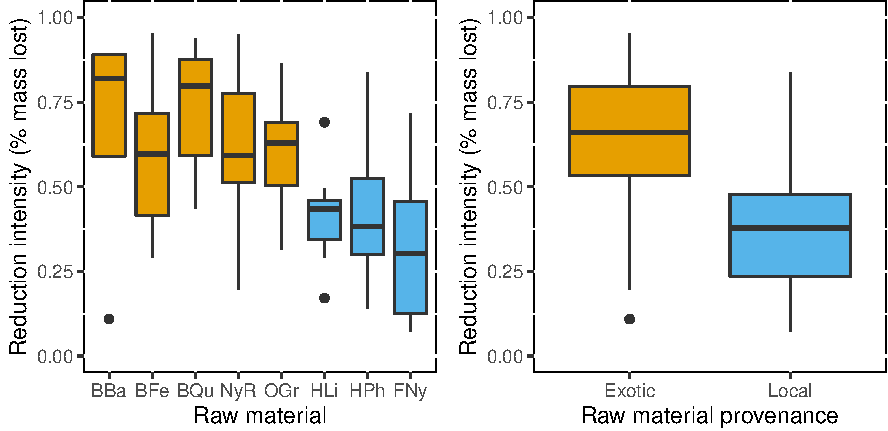
\includegraphics{Kanjera_South_Manuscript_files/figure-latex/fig-3-1.pdf}
\caption{Box plots showing the distribution of core reduction intensity
values as predicted by the generalized linear mixed model
(\hspace{0pt}Douglass et al., 2018\hspace{0pt}). The results show stark
differences in the degree of reduction in materials originating from
more distant sources than those that originate from local sources of
stone. The central bar is the median value (50th percentile). The lower
and upper edges of the box represent the 1st and 3rd quartiles. The
length of the upper whisker reflects the maximum value of the data that
is not 1.5 times greater than the 75th percentile. The length of the
lower whisker is the minimum value of the data not less than 1.5 times
the 25th percentile. The dark circles are observations that are either
1.5 times greater than the 75th percentile or 1.5 times less than the
25th percentile. \label{core_redux_rm}}
\end{figure}

\hypertarget{flake-efficiency}{%
\subsection{2.4 Flake Efficiency}\label{flake-efficiency}}

Flake efficiency was calculated for a subset of flakes included in this
analysis (SOM Table S1). Assuming that most stone tools are produced to
create sharp edges, one possible measure of flake efficiency is
estimating the amount of sharp edge produced per given unit of mass.
Technologies that produced a higher amount of edge per volume of
material can be considered more efficient (\hspace{0pt}Braun and Harris,
2003\hspace{0pt}). Here, we use a measure of edge that is based on
tracing the edge of whole flakes from digital images (\hspace{0pt}Braun
and Harris, 2003\hspace{0pt}). To calculate efficiency, this edge
estimate is divided by the logarithmic transformation of mass
(\hspace{0pt}Braun and Harris, 2003\hspace{0pt}). This transformation is
important when calculating this ratio because mass increases
volumetrically flake edge increases in two dimensions. Thus, the
logarithmic transformation of mass prevents distortions of this ratio
that are size correlated (i.e., allometric). For example, very small
flakes have relatively high edges for a given amount of mass, but this
is not always the most efficient way to produce the greatest amount of
edge relative to volume (e.g., for discussions on this topic, refer to
\hspace{0pt}Kuhn, 1990\hspace{0pt}). Flakes that have long edges
relative to their mass tend to be relatively thin flakes, and there is
the possibility that the efficiency of these tools is limited by their
capabilities to complete certain tasks (e.g., tasks that require
intensive use of edges such as hide scraping may not be feasible with
relatively thin flakes). Here, we calculate the edge-to-mass ratio of
flakes within raw material categories. These values then can be studied
according to raw material type and provenance as aggregate measures are
likely more reflective of the generalized pattern of efficiency in tool
production over time.

\hypertarget{statistical-comparisons}{%
\subsection{2.5 Statistical Comparisons}\label{statistical-comparisons}}

The following statistical comparisons were made to elucidate the broader
land-use strategy of the Kanjera South hominins. To examine the
influence of raw material provenance and transport on core utilization,
core reduction intensity values, flake sequence values, and edge-to-mass
ratio values were compared according to raw material provenience (i.e.,
local versus exotic). The significance of these differences between
local and exotic material was tested using Mann-Whitney U tests as our
data were not normally distributed, and significant differences were
determined using an alpha level of 0.05 (\hspace{0pt}Gotelli and
Ellison, 2013\hspace{0pt}). To determine whether there is relationship
between raw material provenance and the core reduction strategies used
at Kanjera South, the frequency of idealized free-hand reduction types
was compared by raw material type using Fisher's exact test
(\hspace{0pt}Gotelli and Ellison, 2013\hspace{0pt}) because some of the
reduction strategies are represented by 4 or fewer cores. Finally, core
reduction intensity values were also analyzed according to raw material
type. A Kruskal-Wallis test was used to assess the significance of these
differences. All statistical analyses were performed in R v. 3.6
(\hspace{0pt}R Core Team, 2018\hspace{0pt}). Given the number of
quantitative approaches used in this study, we have made the R code and
markdown documents used to conduct this analysis available online.

\hypertarget{results}{%
\section{3 Results}\label{results}}

\hypertarget{core-utilization}{%
\subsection{3.1 Core Utilization}\label{core-utilization}}

Core reduction intensity estimates reveal a wide range of variation in
the amount of mass removed from the cores at Kanjera South. Some cores
were minimally used, whereas others were reduced by as much as 95\% of
their original mass. While there are some differences in the level of
reduction between individual raw material types, the primary differences
are driven by raw material provenance (\hspace{0pt}Fig.
\ref{core_redux_rm}\hspace{0pt}). Cores produced on raw material types
that originate from more distant sources (Bukoban andesite (BBa),
Bukoban felsite (BFe), Bukoban quartzite (BQu), Nyanazian rhyolite
(NyR), and Oyugis granite) are, on average, more substantially reduced
than those that occur locally (fenetized Nyanzian {[}FNy{]}, Homa
phonolite {[}HPh{]}), Homa limestone {[}HLi{]}; Mann-Whitney U, W =
5639.5, p \textless{} .0001; Fig. \ref{core_redux_rm}).

This pattern of core utilization is also reflected in the flake
assemblages. Flake sequence values range from the first flakes
offremoved from the core to the 30th flake in the sequence. The largest
differences are, again, between rock types derived from more distant
sources and those found locally (\hspace{0pt}Fig. 4\hspace{0pt};
Mann-Whitney U, W = \ensuremath{3.3325\times 10^{5}}, p \textless{}
.0001). Flakes produced on rock types from more distant raw material
sources are from later in the reduction sequence, while flakes produced
on raw materials that are available locally are from earlier stages of
reduction (\hspace{0pt}Fig. \ref{flake_seq_rm}\hspace{0pt}).
Interestingly, there is a striking amount of homogeneity in the
distribution of flake sequence values associated with exotic or distant
raw materials. With the exception of BFe, the interquartile range of
flake sequence values is very similar from distant sources. Although BFe
has a wider range than the other exotic materials, its median is quite
similar. The flake sequence values associated with the local materials
are also similar to each other but show slightly more variation.

\begin{figure}
\centering
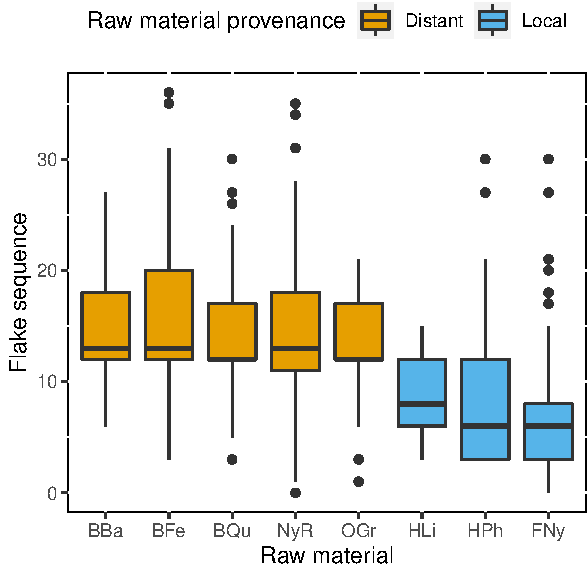
\includegraphics{Kanjera_South_Manuscript_files/figure-latex/fig-4-1.pdf}
\caption{Box plots showing the distribution of flake sequence values
present within the Kanjera South flake assemblage. As is the case with
the core assemblage, the primary differences in flake sequence values
are between materials originating from more distant sources and those
that originate from local sources of stone. The central bar is the
median value (50th percentile). The lower and upper edges of the box
represent the 1st and 3rd quartiles. The length of the upper whisker
reflects the maximum value of the data that is not 1.5 times greater
than the 75th percentile. The length of the lower whisker is the minimum
value of the data not less than 1.5 times the 25th percentile. The dark
circles are observations that are either 1.5 times greater than the 75th
percentile or 1.5 times less than the 25th percentile.
\label{flake_seq_rm}}
\end{figure}

As previously reported, the Kanjera core assemblage comprises a wide
variety of technological types and core reduction strategies
(\hspace{0pt}Braun et al., 2009a\hspace{0pt}). The frequency of core
reduction strategies present has a significant relationship with the raw
material type (Fisher's exact test, p = \ensuremath{5\times 10^{-4}}).
Although unifacial and unidirectional reduction strategies are present
in small frequencies, there is a greater representation of centripetal,
bifacial, and multifacial exploitation strategies in materials from more
distant origins (\hspace{0pt}Fig. \ref{core.tech}). On the other hand,
local materials such as the FNy and HPh are represented by a greater
number of unifacial or unidirectional core reduction strategies
(\hspace{0pt}Fig. \ref{core.tech}\hspace{0pt}). Contrary to this general
pattern, cores produced from some of the local materials (e.g., HLi) are
often multifacially reduced. However, as addressed in the discussion,
this is likely related to the properties of the raw material itself
(Braun et al., 2009). When the core reduction intensity values for each
reduction strategy are considered, unifacial and unipolar cores are
reduced less than bifacial, multifacial, or polyhedral cores
(Kruskal-Wallis, chi-squared = 57.07, p \textless{} .0001`;
\hspace{0pt}Fig. \ref{core.tech}\hspace{0pt}). In other words, core
reduction strategies that require fewer core rotations, such as
unifacial and unidirectional strategies, are less reduced than those
that involved more complex patterns.

\begin{figure}
\centering
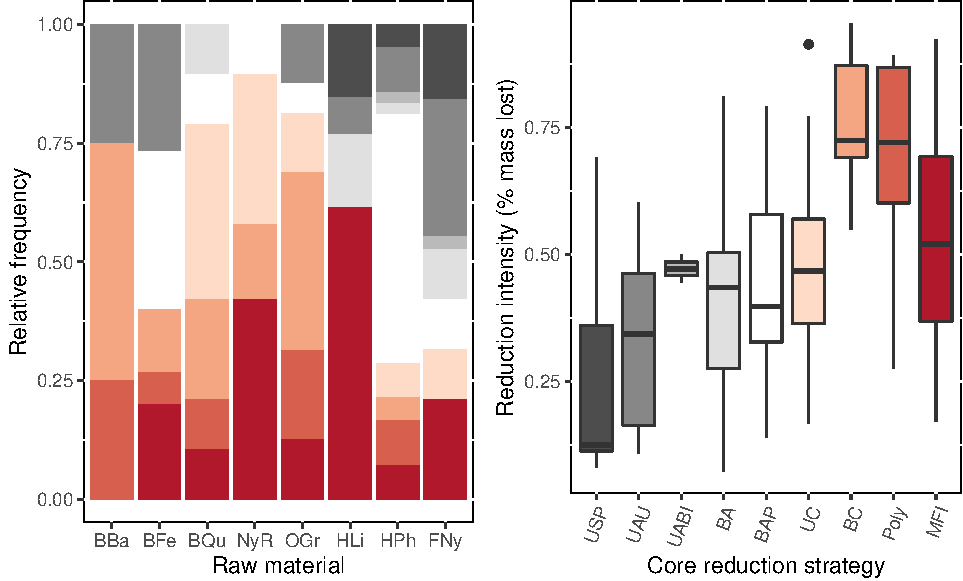
\includegraphics{Kanjera_South_Manuscript_files/figure-latex/fig-5-1.pdf}
\caption{Left: The distribution of core reduction strategies by raw
material type. With the exception of Homa limestone, raw materials that
derive from the Kisi Highlands are more greatly represented by complex
core reduction strategies than those that can be found in the immediate
vicinity of Kanjera South. Right: Box plots showing the distribution of
reduction intensity values according to reduction strategy. The colors
of the boxplots correspond with the representation of different
reduction strategies in the left figure. The central bar is the median
value (50th percentile). The lower and upper edges of the box represent
the 1st and 3rd quartiles. The length of the upper whisker reflects the
maximum value of the data that is not 1.5 times greater than the 75th
percentile. The length of the lower whisker is the minimum value of the
data not less than 1.5 times the 25th percentile. The dark circles are
observations that are either 1.5 times greater than the 75th percentile
or 1.5 times less than the 25th percentile. FNy = feneitized Nyanzian;
HLi = Homa limestone; HPh = Homa phonolite; BBa = Bukoban andesite; BFe
= Bukoban felsite; BQu = Bukoban quartzite; NyR = Nyanzian rhyolite; OGr
= Oyugis granite, USP = unifacial simple partial; UAU = unidirectional
abrupt unifacial; UABI = unifacial abrupt bidirectional; BA =
bidirectional abrupt; BAP = bifacial partial; UC = unifacial
centripetal; BC = bifacial centripetal; Poly = polyhedral; MFI =
mutifacial irregular. \label{core.tech}}
\end{figure}

\hypertarget{flake-efficiency-1}{%
\subsection{3.2 Flake efficiency}\label{flake-efficiency-1}}

Analysis of the relative proportion of flake edge to mass indicates
significantly different technological strategies that were applied to
the different raw materials from the Kanjera South assemblage. Although
the mean values of raw materials are relatively similar, the overall
distribution indicates that rock types from sources that are further
away from Kanjera South (e.g., NyR, BFe, BQu) are produced in a way that
allows for much higher efficiency values than those seen in the rock
types found close to Kanjera South (Mann-Whitney U, W =
\ensuremath{1.91209\times 10^{5}}, p \textless{} .0001). It should be
noted that even though there are significant differences between the
edge-to-mass ratios, the distributions show overlap (\hspace{0pt}Fig.
\ref{flake_efficiency}\hspace{0pt}). This indicates that it is
physically possible to produce flakes with similar edge-to-mass ratios
in each raw material type. Given the results of the core reduction
intensity and flake sequence analysis, it could also be argued that the
observed differences in flake efficiency could simply reflect the
varying levels of reduction intensity observed between the distant and
local assemblage. However, \hspace{0pt}Figure
\ref{flake_efficiency}\hspace{0pt} (right) suggests that there is no
strong relationship between flake sequence and flake efficiency. This
suggests that hominins at Kanjera South did not implement this strategy
as frequently on raw materials that were locally abundant. Hominins at
Kanjera South consistently produced flakes with greater edge and less
mass from rock types that came from more distant sources.

\begin{figure}
\centering
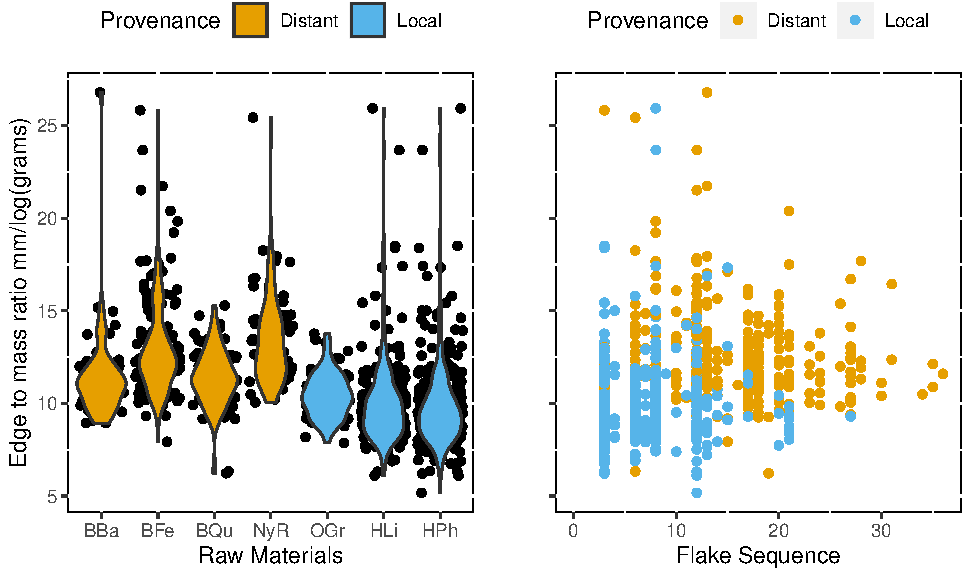
\includegraphics{Kanjera_South_Manuscript_files/figure-latex/fig-6-1.pdf}
\caption{Violin plots showing the distribution of flake efficiency
measures according to raw material. Y axis represents the perimeter of
flakes divided by a logarithmically transformed mass value. Right: A
scatter plot examining the relationship between flake efficiency and
flake sequence. \label{flake_efficiency}}
\end{figure}

\hypertarget{discussion}{%
\section{4 Discussion}\label{discussion}}

\hypertarget{inferring-land-use-at-kanjera-south}{%
\subsection{4.1 Inferring land use at Kanjera
South}\label{inferring-land-use-at-kanjera-south}}

It has long been known that Oldowan archaeological sites represent
points in a dynamic system where stone is both imported and exported
(\hspace{0pt}Isaac, 1984\hspace{0pt}; \hspace{0pt}Toth,
1985\hspace{0pt}; \hspace{0pt}Potts, 1991\hspace{0pt}; \hspace{0pt}Stout
et al., 2005\hspace{0pt}, \hspace{0pt}2010\hspace{0pt};
\hspace{0pt}Semaw, 2006\hspace{0pt}). However, Oldowan sites that are
2.0 Ma or older are situated close to the raw material source (reviewed
in \hspace{0pt}Plummer and Finestone, 2018\hspace{0pt}), whereas Kanjera
South is located more distantly from some sources of material. Thus, the
combination of local and exotic raw materials at Kanjera South allows
for a formal analysis of the stone tool transport process in the early
Oldowan.

The results of this study show an interaction between stone tool
utilization, raw material type, and core reduction strategies. The most
striking distinction is the difference in the degree of utilization of
materials from local and exotic sources. This is also reflected in the
flake sequence data. To some extent, this can be explained by the poor
quality of some of the local materials. As discussed in
\hspace{0pt}Braun et al.~(2009a)\hspace{0pt}, removal sequences in local
feneitized rocks (FNy) tend to be short because of the presence of
preexisting internal fracture planes present in the highly metasomatized
rocks. The chalky nature and block-like geometry of HLi also limits the
number of flakes that can be removed. In contrast, the majority of raw
materials from more distant sources possess fewer flaws and fracture
more predictably than those found locally (\hspace{0pt}Braun et al.,
2009a\hspace{0pt}).

However, not all cores from local sources have internal flaws. In
particular, HPh does not have the defects common in the other local raw
materials but is still less reduced than the nonlocal raw materials. The
coarse-grained nature of Oyugis granite makes it difficult to maintain
angles of less than 90°, thus limiting the degree that the material
could be reduced (\hspace{0pt}Braun et al., 2009a\hspace{0pt}). Despite
these limitations, Oyugis granite is still more reduced than any of the
local raw materials (\hspace{0pt}Fig. 4\hspace{0pt}). The totality of
these data suggests that raw material properties play a role in
reduction intensity but do not explain all the variation in the Kanjera
South assemblage.

The differences in the degree of stone utilization at Kanjera South can
also be interpreted as the result of the continuous use of the
high-quality exotic raw materials as they were moved across long
distances. The higher core reduction intensity values and greater flake
sequence values in the exotic material are consistent with a
distance-decay pattern of tool use that has been documented in a variety
of time periods (\hspace{0pt}Clark, 1979\hspace{0pt};
\hspace{0pt}Newman, 1994\hspace{0pt}; \hspace{0pt}Close,
1999\hspace{0pt}; \hspace{0pt}Blumenschine et al., 2008\hspace{0pt};
\hspace{0pt}Luncz et al., 2016\hspace{0pt}). Although this pattern has
often been associated with a high level of planning and foresight,
modeling work has demonstrated that differences in the reduction
intensity of materials from local and distant sources can arise simply
due to continuous transport even in the absence of a structured land-use
pattern (i.e., random movement; \hspace{0pt}Brantingham,
2003\hspace{0pt}; \hspace{0pt}Pop, 2016\hspace{0pt}). However, the
Kanjera South assemblage deviates from these neutral models in one
critical aspect. These models predict that the variance in tool
reduction intensity will also decrease with distance from the raw
material source (\hspace{0pt}Brantingham, 2003\hspace{0pt}, p.~501). In
contrast with model expectations, while exotic materials are reduced
more substantially than local materials, the interquartile ranges of
flake sequence and core reduction measures of assemblages from distant
sources are as wide (or wider) than those associated with local sources.

Therefore, the Kanjera South assemblage does not fit expectations under
neutral conditions. It has been hypothesized that such deviations from
the neutral model of this nature may arise due to increasingly linear
movements toward specific locations (\hspace{0pt}Brantingham,
2003\hspace{0pt}, \hspace{0pt}2006\hspace{0pt}; \hspace{0pt}Blumenschine
et al., 2008\hspace{0pt}; \hspace{0pt}Braun et al., 2008b\hspace{0pt}).
Moreover, subsequent work modeling the influence of directed movement
toward attractors has shown that while a distance-decay pattern remains
visible, tools from earlier stages of reduction will be over-represented
(i.e., greater variance in reduction (\hspace{0pt}Reeves,
2019\hspace{0pt}). Thus, the greater than expected range in variance in
the reduction intensity of distantly sourced cores may suggest that
hominins directed their movement to Kanjera South. This is not to say
that hominins carried rocks directly to Kanjera South. However, Kanjera
South may have acted as an attractor on the Pleistocene landscape where
hominins frequently visited to carry out stone tool-using behaviors.
This notion is supported to some extent by the fact that the lithics
included in this study were excavated from a 3-m sequence, suggesting
that the patterns evinced by this study are the result of the repeated
visitation by hominins over hundreds to thousands of years.

This attractiveness of Kanjera South is also supported by other
archaeological and paleoecological evidence. Taphonomic studies of the
faunal assemblage from Kanjera South have verified that hominins
efficiently exploited small bovids and may have processed larger
carcasses that were scavenged from carnivores (\hspace{0pt}Ferraro et
al., 2013\hspace{0pt}; \hspace{0pt}Oliver et al., 2019\hspace{0pt}).
Use-wear studies demonstrate that hominins carried out a variety of
resource processing activities with stone artifacts at Kanjera South,
including butchery and the processing of a variety of plants, including
underground storage organs (\hspace{0pt}Lemorini et al.,
2014\hspace{0pt}, \hspace{0pt}2019\hspace{0pt}). These studies suggest
that hominins spent a great deal of time producing stone tools for a
variety of tasks. While the notion that hominins directed their movement
toward specific localities or ecotones has been suggested at other
localities (e.g.~\hspace{0pt}Blumenschine et al., 2008\hspace{0pt},
\hspace{0pt}2012a\hspace{0pt}, \hspace{0pt}2012b\hspace{0pt}), Kanjera
South represents the earliest documented evidence of this pattern. This
reinforces the notion that Oldowan stone tool-use behavior was strongly
integrated into broader foraging strategies of Early Pleistocene
hominins. It may be that this pattern of behavior, as has been suggested
by Potts (1992), is synonymous with the appearance of the Oldowan. This
could be tested by future landscape-scale studies at the earliest
localities such as Ledi-Geraru and Gona (\hspace{0pt}Stout et al.,
2010\hspace{0pt}; \hspace{0pt}Braun et al., 2019\hspace{0pt}).

The land-use pattern elucidated at Kanjera South also differs from
younger Oldowan sites in scale. The movement pattern described at Koobi
Fora (\hspace{0pt}Braun et al., 2008b\hspace{0pt}) suggests that
hominins directed their movements across paleogeographic settings at a
scale of hundreds of meters. At Olduvai Gorge, the directed movement
toward riparian woodlands is thought to have occurred over a scale no
greater than 5 km (\hspace{0pt}Blumenschine et al., 2008\hspace{0pt},
\hspace{0pt}2012a\hspace{0pt}). The data presented here imply that a
pattern of directed movement occurred at a scale of at least 10--13 km
for nonlocal materials. This is an interesting distinction because
Kanjera South is one of the few sites from this time frame situated in
an open grassland (\hspace{0pt}Plummer et al., 2009b\hspace{0pt}).
Modern humans tend to travel farther and more frequently in open arid
environments than those who live in more closed habitats
(\hspace{0pt}Kelly, 2007\hspace{0pt}; \hspace{0pt}Burnside et al.,
2012\hspace{0pt}). Savanna-adapted chimpanzees from Fongoli, Senegal,
also possess a larger home range and practice fission-fusion less
frequently (\hspace{0pt}Pruetz and Bertolani, 2009\hspace{0pt}). In this
respect, the increased scale of this structured land-use pattern at
Kanjera South may further attest to the adaptive flexibility of Oldowan
hominin open environments.

\hypertarget{the-influence-of-land-use-on-oldowan-production-strategies}{%
\subsection{4.2 The influence of land use on Oldowan production
strategies}\label{the-influence-of-land-use-on-oldowan-production-strategies}}

The results of this study also suggest that patterns of land use
influence the technical decisions of Oldowan tool makers. At Kanjera
South, exotic raw materials show a strong bias toward more reduced,
complete bifacial and multifacial reduction strategies, as opposed to
the more even representation of core reduction strategies among local
materials. This suggests that the broader pattern of stone tool
transport influenced the ways in which Oldowan hominins economized
stone. The relatively long transport distance, in combination with the
lower quality of material available near Kanjera South, may have
incentivized the retention of exotic raw materials in areas where
lithologies of such quality were less abundant. In this light, the high
frequency of bifacial and multifacial reduction strategies and the
higher cutting edge-to-mass ratios present in the exotic raw materials
may reflect a general need to maximize the utility that could be
extracted from these cores. The exploitation of multiple flake removal
surfaces allows a core to remain active in a tool kit for a longer
period.

In contrast, the predominantly unifacial and partial bifacial reduction
strategies in combination with the significantly lower edge-to-mass
ratio values may reflect a more expedient treatment of the lower quality
local raw materials. However, it must also be noted that some of the
technical variation within the local assemblage likely reflects the
constraints imposed by the quality of the raw material. The predominance
of irregular multifacial strategies in the HLi is argued to be the
result of its chalky nature and block-like geometry (\hspace{0pt}Braun
et al., 2009a\hspace{0pt}). Therefore, this corpus of information may
indicate that Oldowan hominins were able to adopt different technical
strategies to mitigate the changing qualities in available raw materials
over large transport distances. This pattern of exploitation, in the
context of the broader land-use strategy at Kanjera South, provides
additional evidence for a high level of planning and foresight in
Oldowan hominins.

These results also have broader implications for how techno-economic
variation arises in the Oldowan record. The variability in the Oldowan
record is often interpreted through a socio-cognitive lens, in which
technological differences between assemblages are argued to reflect
socially learned information that particularize various groups or
individuals (\hspace{0pt}Delagnes and Roche, 2005\hspace{0pt};
\hspace{0pt}Roche et al., 2009\hspace{0pt},
\hspace{0pt}2018\hspace{0pt}; \hspace{0pt}Stout, 2011\hspace{0pt};
\hspace{0pt}Stout et al., 2019\hspace{0pt}). More recently, these
criteria have been used to argue for the presence of copying social
learning mechanisms in the earliest Oldowan (\hspace{0pt}Stout et al.,
2019\hspace{0pt}). However, the results of this study strongly link the
application of various technical strategies with the broader land-use
system in which tool use is incorporated. Moreover, the fact that core
reduction intensity seems to increase as cores are increasingly rotated
further suggests that unifacial, bifacial, and multifacial cores may not
reflect discrete strategies but are rather points on continuum of
reduction that arise out of a need to maximize the utility of
high-quality materials.

The notion that Oldowan stone tool variation may reflect a continuum of
utilization has been previously suggested based on evidence from
controlled least effort experiments by \hspace{0pt}Toth
(1982)\hspace{0pt} and later by \hspace{0pt}Moore and Perston
(2016)\hspace{0pt}. \hspace{0pt}Potts (1991)\hspace{0pt} suggested that
this also may be the case with cores at Olduvai Gorge by showing how
different core types varied according to mass. By directly estimating
the amount of mass lost from each core in the assemblage, we find
further support for this notion as the various core exploitation
strategies present at Kanjera South are correlated with reduction
intensity. In light of the results of this study, the frequent use of
unifacial reduction strategies at sites such as Lokalelei 2C, East Gona,
Hadar, Omo, and Ledi-Geraru may relate to the overall abundance of
knappable material that is immediately available at these sites
(\hspace{0pt}Kimbel et al., 1996\hspace{0pt}; \hspace{0pt}Roche et al.,
1999\hspace{0pt}; \hspace{0pt}Stout et al., 2005\hspace{0pt};
\hspace{0pt}Braun et al., 2019\hspace{0pt}).

Finally, while the preceding analysis emphasizes the role of the broader
environment and land use on technological variability, ecology is not
the sole driver of Oldowan technical variation. The interquartile ranges
in \hspace{0pt}Figure 6\hspace{0pt} show a substantial amount of overlap
between the reduction intensity and core reduction strategies. This
suggests that not all variation can be explained by environmental
parameters such as raw material availability and material properties.
Moreover, at other localities (e.g.~West Turkana), intersite differences
are not easily explained by factors such as raw material availability
alone (\hspace{0pt}Roche et al., 2018\hspace{0pt}). This unexplained
variation may be the result of socio-cultural dynamics that may have
maintained information regarding the stone tool production process
between groups. However, the fidelity and the mechanisms that underlie
the maintenance of this information remain an open debate
(\hspace{0pt}Hovers, 2012\hspace{0pt}; \hspace{0pt}Morgan et al.,
2015\hspace{0pt}; \hspace{0pt}Tennie et al., 2016\hspace{0pt},
\hspace{0pt}2017\hspace{0pt}; \hspace{0pt}Stout et al.,
2019\hspace{0pt}). Nevertheless, the application of quantitative
measures of core reduction intensity, flake sequence, and edge-to-mass
ratio, in combination with broader contextual information regarding raw
material quality and provenance, further elucidates the relationship
between hominin land use and Oldowan technical decision-making.

\hypertarget{conclusion}{%
\section{Conclusion}\label{conclusion}}

The Oldowan industrial complex reflects a complex interaction of
ecological, behavioral, and social factors. The combination of
quantitative measures of stone tool reduction with qualitative
characterizations of lithic technology (e.g., Braun et al., 2009;
\hspace{0pt}Plummer and Bishop, 2016\hspace{0pt}) provides new insights
into the ecological factors that influence Oldowan technology and
hominin behavior. At Kanjera South, exotic materials are more
substantially reduced than local materials, reflecting differences in
the quality of the lithologies available. The durability and hardness of
exotic materials (\hspace{0pt}Braun et al., 2009a\hspace{0pt}) would
have incentivized their transport over longer distances
(\hspace{0pt}Braun et al., 2008a\hspace{0pt}). Differences in reduction
intensity highlight that Oldowan tools were part of a mobile tool kit
that reflects a broader land-use strategy. The marked differences in
reduction intensity in combination with the paucity of early sequence
flakes suggest that exotic materials were often used before their
arrival at Kanjera South. Although exotic materials are more reduced
than local materials, the variance in the amount of stone tool reduction
does not adhere to neutral expectations. This result suggests that the
lithic assemblage at Kanjera South reflects a structured land-use
pattern where hominins may have directed their movement, at least on
occasion, to Kanjera South.

This pattern of stone tool transport and use also appears to have
influenced the technological strategies used by Oldowan tool makers at
Kanjera South. The relationship between core reduction strategies and
reduction intensity indicates that raw material quality and provenance
have a strong influence on the technological variation observed within a
lithic assemblage. While these results show that ecological parameters
have a strong effect on stone tool variation, a substantial amount of
variation remains unexplained by ecology alone. Future studies would
benefit from an integrated approach to understand the behavioral
significance of the Oldowan.

\hypertarget{acknowledgments}{%
\section{Acknowledgments}\label{acknowledgments}}

The authors thank the National Museums of Kenya and M. Kibunjia, F.K.
Manthi, R. Kinyanjui, J. Kibii, and E. Ndiema for support. J.M. Nume and
B. Onyango managed the Kanjera field teams. The authors acknowledge
Kenya Government permission granted by the Ministry of Sports, Culture
and the Arts and by NACOSTI permit P/14/7709/701. Funding from the
L.S.B. Leakey Foundation, the National Geographic Society, the National
Science Foundation, the Wenner-Gren Foundation, and the Professional
Staff Congress--City University of New York Research Award Program to
T.W.P. for Kanjera field and laboratory work is gratefully acknowledged.
The authors would like to thank Rick Potts and the Human Origins Program
at the Smithsonian Institution for support during all phases of the
Kanjera research and the Peter Buck Fund for Human Origins Research. The
authors report no competing interests.

\hypertarget{references}{%
\section*{References}\label{references}}
\addcontentsline{toc}{section}{References}

\hypertarget{refs}{}
\begin{CSLReferences}{1}{0}
\leavevmode\hypertarget{ref-braunEarliestKnownOldowan2019}{}%
Braun, D.R., Aldeias, V., Archer, W., Arrowsmith, J.R., Baraki, N.,
Campisano, C.J., Deino, A.L., DiMaggio, E.N., Dupont-Nivet, G., Engda,
B., Feary, D.A., Garello, D.I., Kerfelew, Z., McPherron, S.P.,
Patterson, D.B., Reeves, J.S., Thompson, J.C., Reed, K.E., 2019.
Earliest known {Oldowan} artifacts at \&gt;2.58 {Ma} from
{Ledi}-{Geraru}, {Ethiopia}, highlight early technological diversity.
Proceedings of the National Academy of Sciences. 116, 11712--11717.

\leavevmode\hypertarget{ref-braunOldowanTechnologyRaw2009}{}%
Braun, D.R., Plummer, T.W., Ditchfield, P.W., Bishop, L.C., Ferraro,
J.V., 2009. Oldowan {Technology} and {Raw Material Variability} at
{Kanjera South}. In: Interdisciplinary {Approaches} to the {Oldowan},
Vertebrate {Paleobiology} and {Paleoanthropology}. {Springer
Netherlands}, {Dordrecht}, pp. 99--110.

\leavevmode\hypertarget{ref-delatorreOmoRevisitedEvaluating2004}{}%
de la Torre, I., 2004. Omo {Revisited}: {Evaluating} the {Technological
Skills} of {Pliocene Hominids}. Current Anthropology. 45, 439--465.

\leavevmode\hypertarget{ref-delagnesLatePlioceneHominid2005}{}%
Delagnes, A., Roche, H., 2005. Late {Pliocene} hominid knapping skills:
{The} case of {Lokalalei 2C}, {West Turkana}, {Kenya}. Journal of Human
Evolution. 48, 435--472.

\leavevmode\hypertarget{ref-ditchfieldGeochronologyPhysicalContext2019}{}%
Ditchfield, P.W., Whitfield, E., Vincent, T., Plummer, T., Braun, D.,
Deino, A., Hertel, F., Oliver, J.S., Louys, J., Bishop, L.C., 2019.
Geochronology and physical context of {Oldowan} site formation at
{Kanjera South}, {KenyaP}. {W}. {DITCHFIELD AND OTHERSPhysical} setting
of {Oldowan} site at {Kanjera South}, {Kenya}. Geological Magazine. 156,
1190--1200.

\leavevmode\hypertarget{ref-goldman-neumanRawMaterialSelectivity2012}{}%
Goldman-Neuman, T., Hovers, E., 2012. Raw material selectivity in {Late
Pliocene Oldowan} sites in the {Makaamitalu Basin}, {Hadar}, {Ethiopia}.
Journal of Human Evolution. 62, 353--366.

\leavevmode\hypertarget{ref-plummerResearchLatePliocene1999}{}%
Plummer, T.W., Bishop, L.C., Ditchfield, P.W., Hicks, J., 1999. Research
on {Late Pliocene Oldowan Sites} at {Kanjera South}, {Kenya}. Journal of
Human Evolution. 36, 151--170.

\leavevmode\hypertarget{ref-semawWorldOldestStone2000}{}%
Semaw, S., 2000. The {World}'s {Oldest Stone Artefacts} from {Gona},
{Ethiopia}: {Their Implications} for {Understanding Stone Technology}
and {Patterns} of {Human Evolution Between} 2{\(\cdot\)}6{\(\cdot\)}5
{Million Years Ago}. Journal of Archaeological Science. 27, 1197--1214.

\leavevmode\hypertarget{ref-stoutRawMaterialSelectivity2005}{}%
Stout, D., Quade, J., Semaw, S., Rogers, M.J., Levin, N.E., 2005. Raw
material selectivity of the earliest stone toolmakers at {Gona}, {Afar},
{Ethiopia}. Journal of Human Evolution. 48, 365--380.

\leavevmode\hypertarget{ref-tothOldowanCaseStudies2006}{}%
Toth, N., Schick, K., 2006. The {Oldowan}: {Case Studies} into the
earliest {Stone Age}. {Stone Age Institute Press}, {Bloomington}.

\end{CSLReferences}


\end{document}
